\chapter{Control Óptimo de Sistemas Lineales}

\section{Planteamiento (caso particular)}

Dado un sistema dinámico LTI:

\begin{align*}
    \dot{x}(t) = A x(t) + B u(t)
\end{align*}

Asumiendo que el sistema LTI es:

\begin{itemize}
    \item estable y controlable, o
    \item inestable, pero los estados inestables son controlables $\Longrightarrow$ estados estabilizables.
\end{itemize}

El problema es encontrar $u(t)$, para llevar el estado $x(t)$ hasta $x(t_1)$, para un tiempo finito $t\in[t_0,t_1]$, tal que se cumpla la siguiente condición, donde $J(u)$ es el funcional de desempeño:

\begin{align*}
    J(u) = \int_{t_0}^{t_1} l \big( x(t), u(t), t \big) dt + m \big( x(t_1) \big)
\end{align*}

\begin{itemize}
    \item $\int_{t_0}^{t_1}l\big(x(t),u(t),t\big)dt$: ``Costo de viaje'' (running cost)
    \item $m\big(x(t_1)\big)$: costo terminal
\end{itemize}

El problema de control óptimo se define como:

\begin{align*}
    u^\star = \arg \min_u J(u)
\end{align*}

\section{Control LQR de horizonte infinito (tiempo contínuo)}

Dado el sistema dinámico LTI de tiempo contínuo:

\begin{align*}
    \dot{x} = A x(t) + B u(t), \qquad x(0) = x_0
\end{align*}

Ahora el problema es encontrar $u(t)$, para llevar los estados $x(t)$ hasta $0$ en un horizonte de tiempo infinito $t \in [0,\infty)$, tal que el funcional de desempeño:

\begin{align*}
    J(u)=\int_{0}^{\infty} \left(x^T Q x+u^T R u \right) dt
\end{align*}

se mininice:

\begin{align*}
    u^\star = \arg \min_u J(u)
\end{align*}

donde $Q$ y $R$ son matrices definidas positivas y simétricas. Notar que en este caso de LQR de horizonte infinito se asume que el costo terminal es cero.\\

Cabe mencionar que matrices $Q$ y $R$ penalizan los estados y control, respectivamente, en el cálculo del funcional de desempeño. Esto quiere decir que valores grandes de $Q$ priorizan más la minimización de los estados, mientras que valores grandes de $R$ priorizan señales de control con menor esfuerzo (por ejemplo, menor consumo energético).

Supongamos que la matriz $P$ es cuadrada, simétrica ($P = P^T$) y definida positiva ($P \succ 0$), y que se agrega el término $x_0^T P x_0$ explícitamente al funcional de desempeño sin cambiar su estructura original:

\begin{align*}
    J(u) &= \underbrace{\left( x_0^T P x_0 - x_0^T P x_0 \right)}_{=0} + \int_{0}^{\infty} \left(x^T Q x+u^T R u \right) dt \\
    & = x_0^T P x_0 - x_0^T P x_0 + \int_{0}^{\infty} \left(x^T Q x+u^T R u \right) dt
\end{align*}

Ahora, utilizando el \emph{teorema fundamental del cálculo}, la siguiente igualdad se cumple:

\begin{subequations}
\begin{align}
    \int_{0}^{\infty} \frac{d}{dt}\left( x^T P x\right) dt &= x_\infty^T P x_\infty - x_0^T P x_0 \\
                              &= 0 - x_0^T P x_0
\end{align} 
\end{subequations}

Reemplazando en el funcional de desempeño:

\begin{align}
    J(u) &= x_0^T P x_0 + \int_{0}^{\infty} \left[\frac{d}{dt}\left( x^T P x\right) + x ^T Q x+u^T R u \right] dt
\end{align}

Desarrollando el primer término dentro de la integral utilizando la regla de la cadena:

\begin{align}
    \frac{d}{dt}\left( x^T P x\right) = \dot{x}^T P x + x^T P \dot{x}
\end{align}

Reemplazando la ecuación de estados:

\begin{align}
    \frac{d}{dt}\left( x^T P x\right) &= \left(A x + B u\right)^T P x + x^T P \left(A x + B u\right)\\
    &= x^T A^T P x + u^T B^T P x + x^T P A x + x^T P B u \\
    &= x^T \left( A^T P + PA\right) x + 2 u^T B^T P x \\
\end{align}

Reemplazando en el funcional de desempeño:

\begin{align}
    J(u) &= x_0^T P x_0 + \int_{0}^{\infty} \left[ x^T \left( A^T P + PA + Q\right) x + u^T R u  + 2 u^T B^T P x \right] dt
\end{align}

Utilizando la técnica de ``completar los cuadrados'':

\begin{subequations}
\begin{align}
    \left( u + K x\right)^T R \left( u + K x\right) = u^T R u + 2 u^T R K x + x^T K^T R K x \\
    \Rightarrow  u^T R u + 2 u^T R K x =  \left( u + K x\right)^T R \left( u + K x\right) - x^T K^T R K x
\end{align}   
\end{subequations}

Igualando $K = R^{-1} B^T P$:

\begin{align}
    u^T R u + 2 u^T B^T P x =  \left( u + R^{-1} B^T P x\right)^T R \left( u + R^{-1} B^T P x\right) - x^T \left(P^T B R^{-1} B^T P \right) x
\end{align}

Nuevamente reemplazamos en el funcional de desempeño:

\begin{align}
    J(u) &= x_0^T P x_0 + \int_{0}^{\infty} \left[ x^T \left( A^T P + PA + Q - P^T B R^{-1} B^T P\right) x + \left( u + R^{-1} B^T P x\right)^T R \left( u + R^{-1} B^T P x\right) \right] dt
\end{align}

Notas:

\begin{enumerate}
    \item Término fuera de la integral $x_0^T P x_0$ es constante, y solo depende de las condiciones iniciales.
    \item Ambos términos dentro de la integral son formas cuadráticas.
    \item Si $A^T P + PA + Q - P^T B R^{-1} B^T P \succeq 0$, entonces primer término de la integral es mayor o igual que cero.
    \item Dado que $R \succ 0$ (definida positiva), el segundo término de la integral ya es mayor o igual que cero.
    \item Por lo tanto, el funcional de desempeño $J(u) \geq x_0^T P x_0$.
    \item Minimizar $J(u)$ implica que los términos de la integral deben ser cero.
    \item Primer término es cero ssi $A^T P + PA + Q - P^T B R^{-1} B^T P = 0, \forall x(t) \neq 0$.
    \item Segundo término es cero ssi $u(t) - R^{-1} B^T P x(t) =0$, ya que $R \succ 0$.
\end{enumerate}

Finalmente derivamos las ecuaciones que deben cumplirse para el control óptimo LQR de horizonte infinito:

\begin{align}
    J(u^\star(t)) = x_0^T P x_0 \\
    u^\star(t) = - K x(t) \\
    A^T P + PA + Q - P^T B R^{-1} B^T P = 0 \label{eq:ARE}
\end{align}

Entonces, la ganancia del controlador LQR horizonte infinito, $K = R^{-1} B^T P$, se calcula resolviendo primero la ecuación algebraica de Ricatti \eqref{eq:ARE} para obtener el valor de $P$. \\

En Matlab, se utiliza la función \texttt{lqr()}.

\begin{figure}[H]
    \centering
    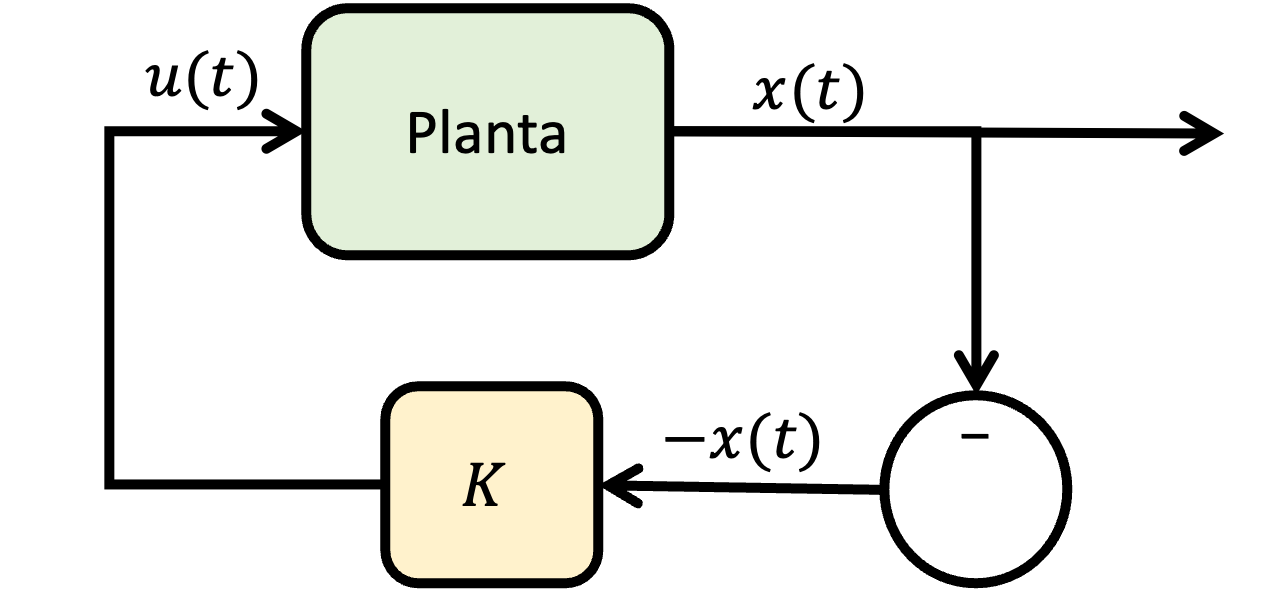
\includegraphics[width=3in]{Figuras/statefeedback.png}
\end{figure}

\section{Heurística de diseño}

\par P: ¿Cómo elijo los valores de $Q$ y $R$? 
\par R: Recordar que

\begin{align*}
    J(u) = \int_0^\infty \Big( x^T Qx+u^T Ru\Big) dt
\end{align*}

\par Recordar que en sistemas estructurales:

\begin{align*}
    x = \left[
    \begin{array}{c}
     \dot{z} \\ \dot{z} 
    \end{array}\right]
\end{align*}

\begin{itemize}
    \item $z$: desplazamiento
    \item $\dot{z}$: velocidad
\end{itemize}

Podemos escribir la forma cuadrática $x^T Q x$ de manera tal que le asignamos un significado físico:

\begin{align*}
    \frac{1}{2}x^T Qx=\frac{1}{2}\left[
    \begin{array}{cc}
     \dot{z} & \dot{z} 
    \end{array}\right] \left[
    \begin{array}{cc}
     K_s & 0 \\ 0 & M_s 
    \end{array}\right] \left[
    \begin{array}{c}
     \dot{z} \\ \dot{z} 
    \end{array}\right] = \frac{1}{2}z^T K_s z+\frac{1}{2}\dot{z}^T M\dot{z}
\end{align*}

\begin{itemize}
    \item $\frac{1}{2}z^T K_s z$: Energía potencial
    \item $\frac{1}{2}\dot{z}^T M \dot{z}$: Energía cinética
\end{itemize}

Por otra parte: $u^T Ru$: energía consumida por el controlador.

\par \underline{Comentario}: No importan los valores absolutos de $Q$ y $R$ en el resultado del control óptimo. Lo que s;i importan son los valores relativos de $Q$ respecto a $R$ (o viceversa).

\begin{align*}
    J(u)=\int_0^\infty (x^T Q x + u^T R u)dt
\end{align*}

\begin{itemize}
    \item $Q$ es mayor que $R$: resultado es sensible a los estados. \\
    \underline{Nota}: Si $R\to 0$: control ``barato'' (cheap) LQR. No es recomendable. \\
    $K=R^{-1}B^T P$: valor muy grande.
    \item $R$ es mayor que $Q$: resultado es sensible a la señal de control.
\end{itemize}

\subsection{Regla de Bryson}

Elegir $Q$ y $R$ matrices diagonales. Cada componente de $q_{ii}$ y $r_{ii}$ están dados por:

\begin{align*}
    q_{ii} &= \frac{1}{\text{máx valor aceptable de }x_i^2}\\
    r_{ii} &= \frac{1}{\text{máx valor aceptable de }u_i^2}
\end{align*}

\section{Filtro de Kalman (tiempo contínuo)}

Sea el sistema LTI de tiempo contínuo:

\begin{align*}
    \dot{x} &= Ax+B_u u +B_w w(t)\\
    y &= Cx+v(t)
\end{align*}

donde $w(t)$ es la perturbación sobre el sistema y $v(t)$ es el ruido de la medición.\\

\begin{figure}[H]
    \centering
    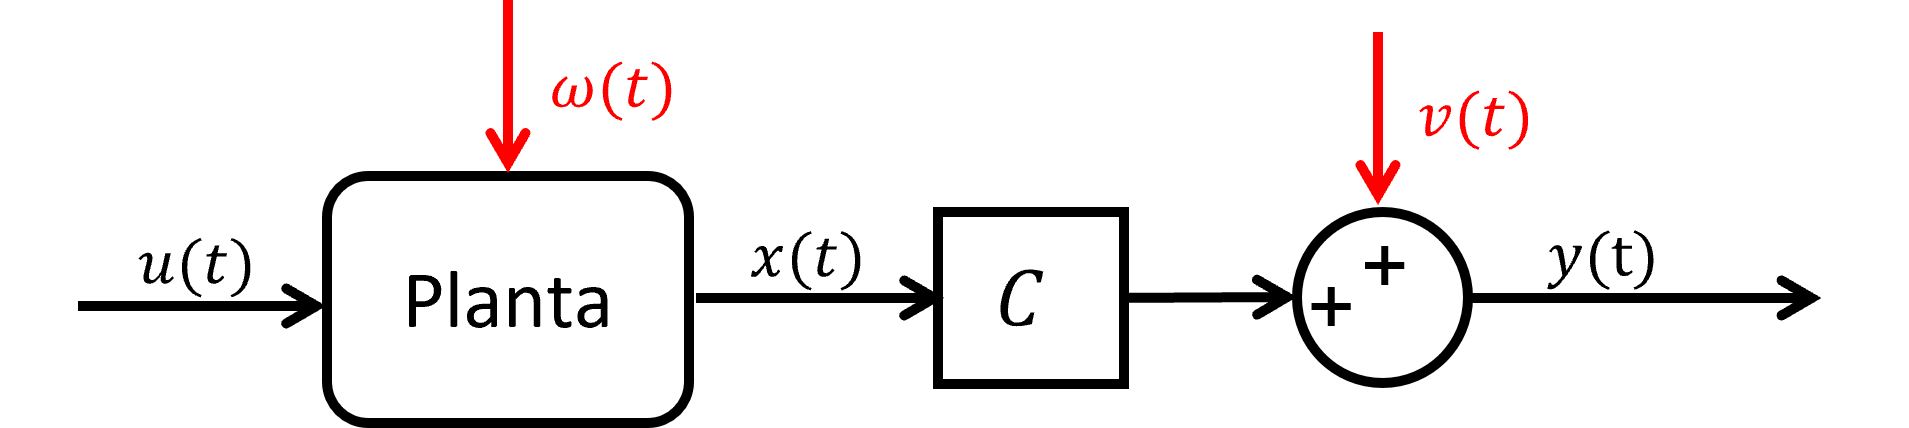
\includegraphics[scale=0.7]{Figuras/wv.png}
\end{figure}

\par \underline{Objetivo}: Estimar los estados $x$ utilizando un observador óptimo $\Longrightarrow$ Filtro de Kalman.\\

\par \underline{Condición}: 

\begin{itemize}
    \item $(C,A)$ es observable
    \item $A$ es Hurwitz
    \item $\Longrightarrow$ Estados detectables
\end{itemize}

Asumir que $w(t)$ y $v(t)$ son p.e. Gaussianos, w.s.s., y de media cero:

\begin{itemize}
    \item Perturbación, $w(t)$: \begin{itemize}
        \item $\mathbb{E}\{w(t)\}=0$
        \item $\mathbb{E}\{w(t) w^T (s)\}=Q_w \delta(t-s)$
    \end{itemize}
    \item Ruido, $v(t)$: \begin{itemize}
         \item $\mathbb{E}\{v(t)\}=0$
        \item $\mathbb{E}\{v(t) v^T (s)\}=R_v \delta(t-s)$
    \end{itemize}
\end{itemize}

Asumir en el caso particular que:

$$\mathbb{E}\{w(t)v^T (s)\}=0 \Longrightarrow \text{$w(t)$ y $v(t)$ están descorrelacionados.}$$

% \begin{figure}[H]
%     \centering
%     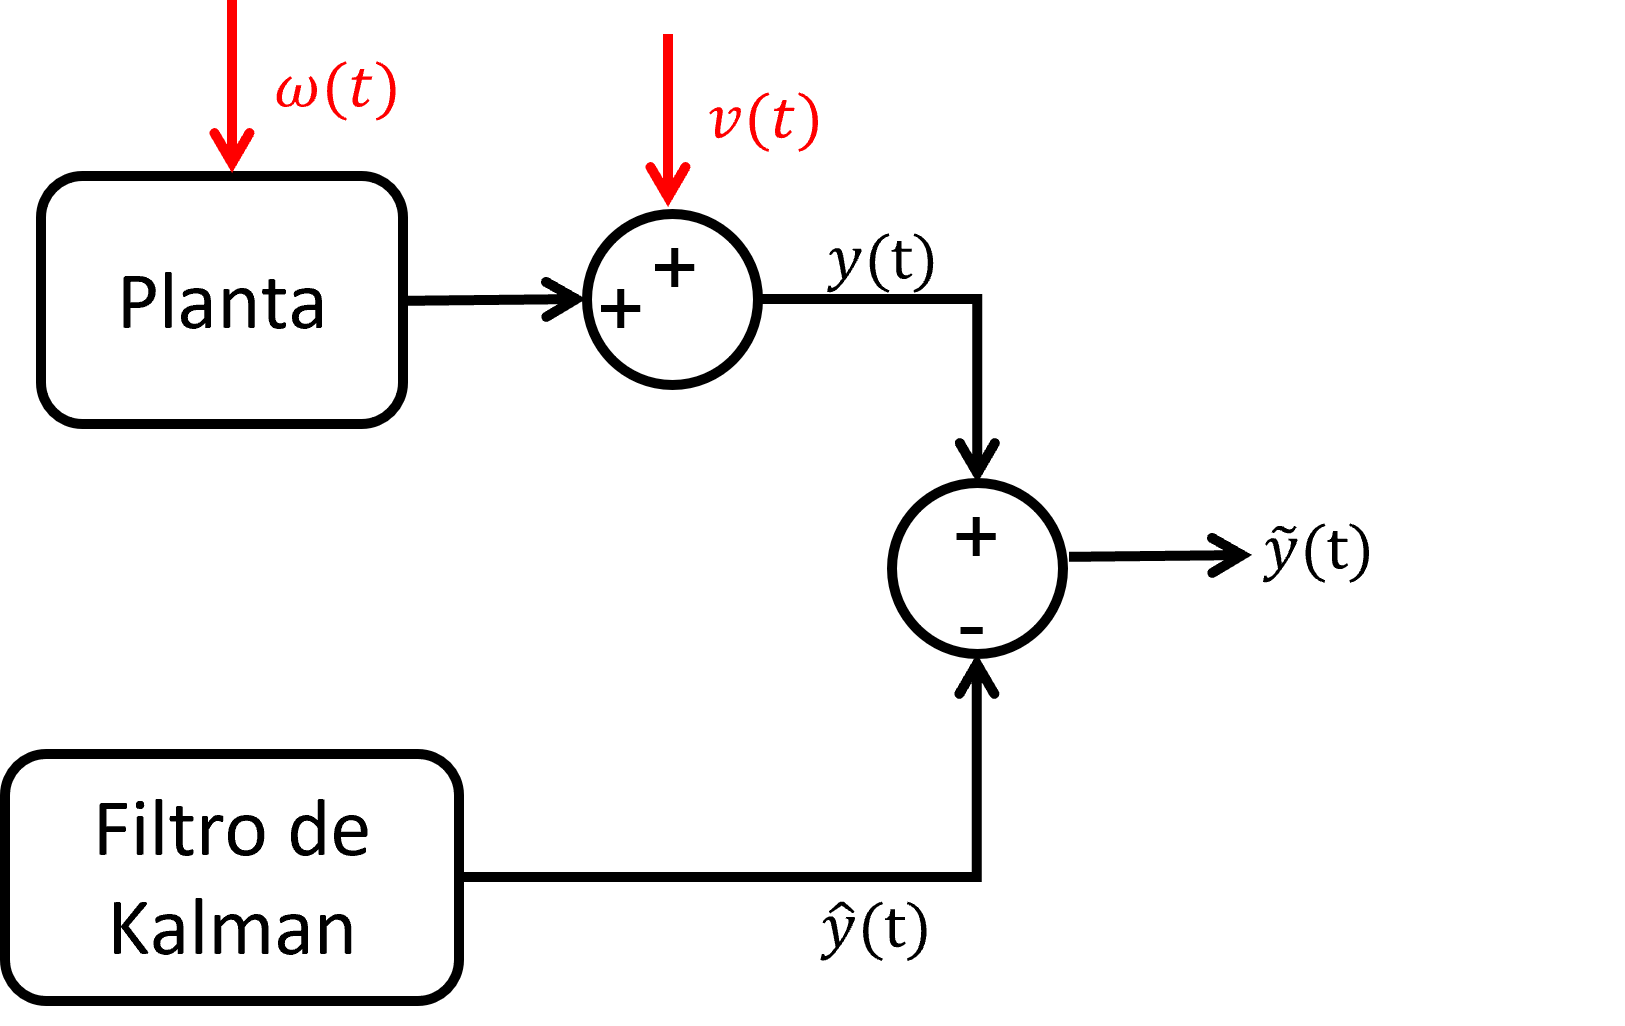
\includegraphics[scale=0.7]{Figuras/Kalman.png}
% \end{figure}

\par Problema de optimización: 

\begin{align*}
    \text{Minimizar } \tilde{y} &= y-\hat{y}\\
    \Leftrightarrow \text{Minimizar } \tilde{x} &= x - \hat{x}
\end{align*}

\underline{Definición}: Matriz de autocovarianza del error de estado $\tilde{x}$ (en estado estacionario) 

\begin{align*}
    \Gamma=\mathbb{E}\{\tilde{x}\tilde{x}^T \} \text{: matriz cuadrada, simétrica, definida positiva}
\end{align*}

\underline{Problema}: $\min J$, $J=\text{trace}(\Gamma^T \Gamma)$

$$J=\mathbb{E} \Bigl\{[x_i-\hat{x}_i][x_i-\hat{x}_i]\Bigr\} $$

Los pasos a seguir son análogos al problema de control óptimo LQR de horizonte infinito. 

\begin{enumerate}
    \item La ganancia de Kalman se define como: $L = \Gamma C^T R_v ^{-1}$
    \item $\Gamma$ se obtiene de resolver la siguiente ecuación algebraica de Riccati.
\end{enumerate}

\begin{align}
    A \Gamma + \Gamma A^T + B_w Q_w B_w^T - \Gamma C^T R_v^{-1} C \Gamma = 0
\end{align}

En términos prácticos, este problema se resuelve en Matlab mediante el comando \texttt{kalman()}

$$(L_{KAL},\Gamma)=\text{Kalman}(A,C,Q_\omega,R_v) $$

Finalmente:

\begin{align*}
    \dot{\hat{x}} &= A \hat{x} + B_u u + L \tilde{y} \\
    \hat{y} &= C\hat{x}
\end{align*}

\begin{figure}[H]
    \centering
    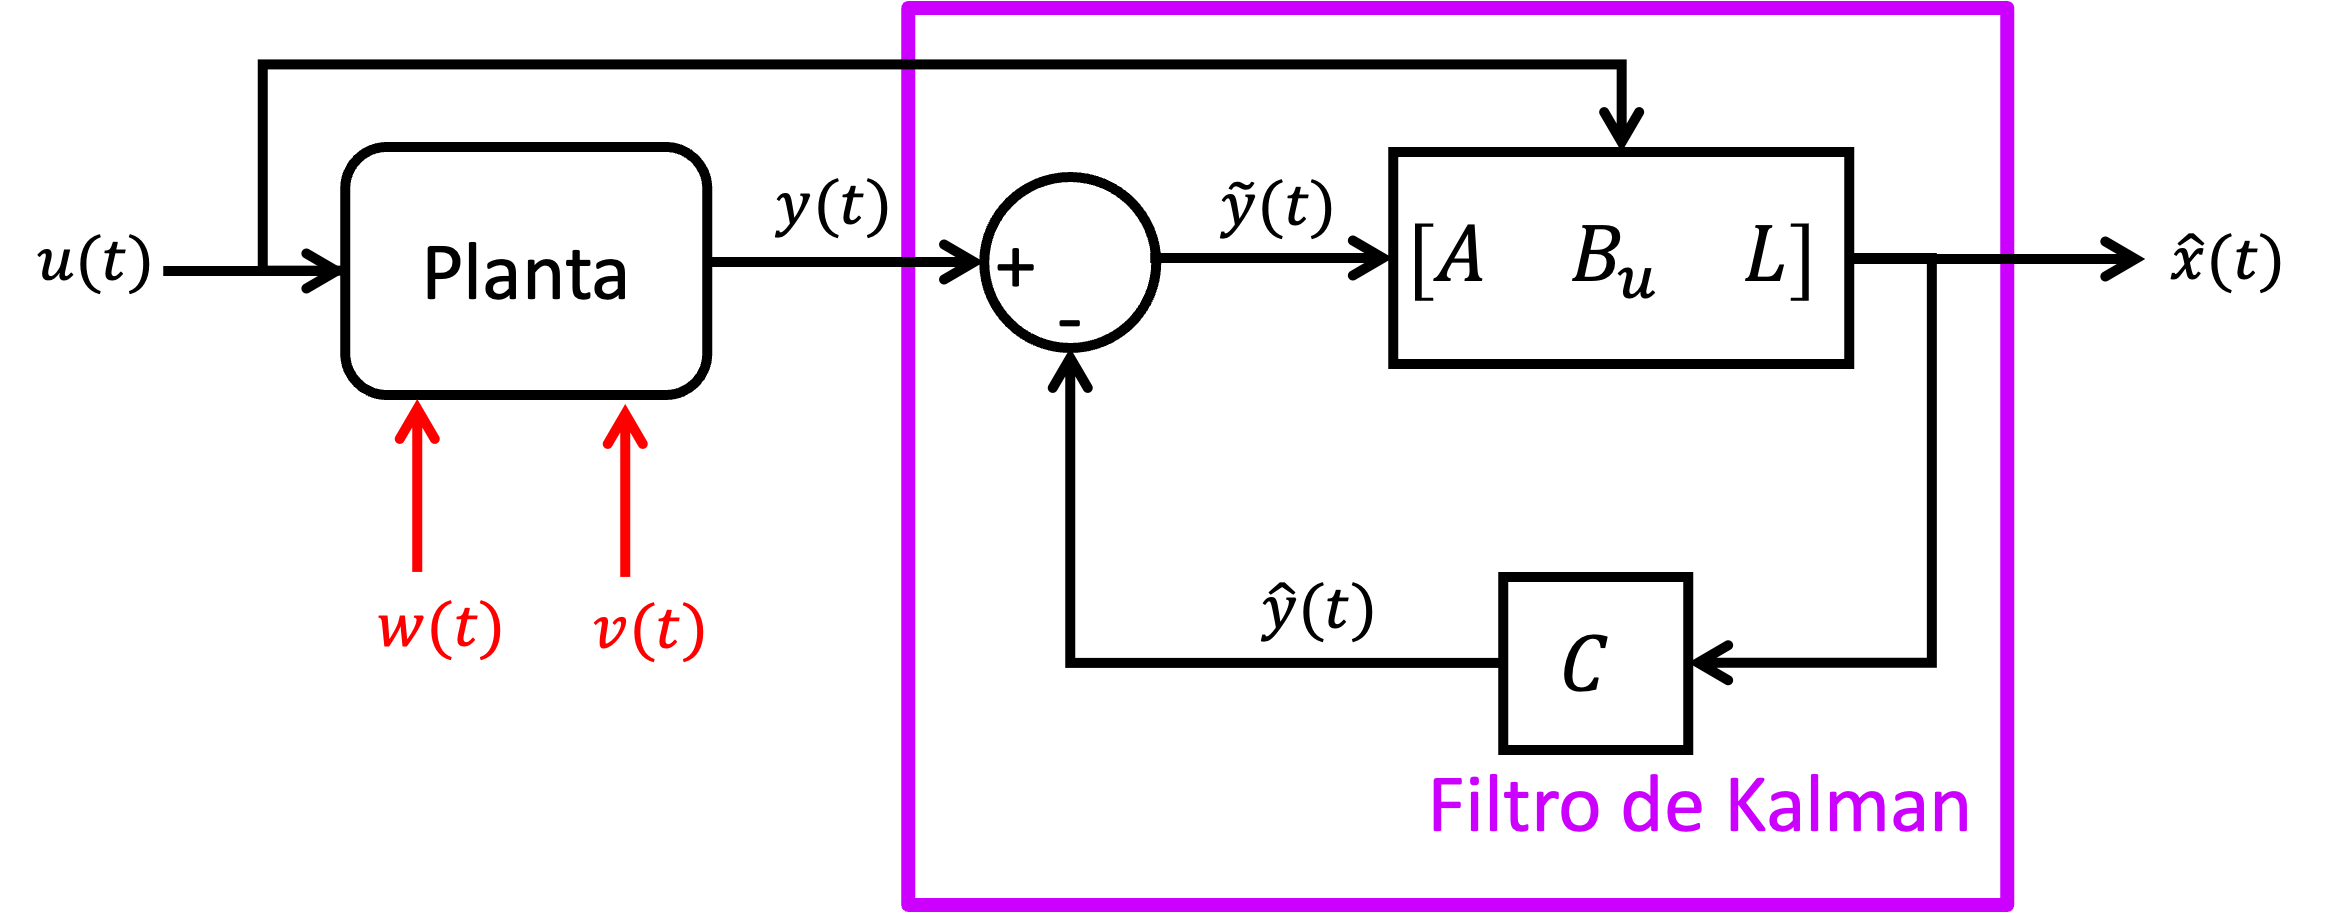
\includegraphics[width=5in]{Figuras/kalman_v2.png}
\end{figure}

\section{Control LQG (tiempo contínuo)}

LQG = Linear Quadratic Gaussian\\

\par Suponga el sistema LTI:

\begin{align*}
    \dot{x} &= Ax + B_u u +B_w w\\
    y &= C x + v
\end{align*}

\underline{Objetivo}: diseñar un controlador óptimo con información de la respuesta.

\begin{align*}
    \text{Control óptimo (LQR)} + \text{Obervador óptimo (Kalman)} \overset{\text{Principio de superposición}}{=} LQG
\end{align*}

\begin{figure}[H]
    \centering
    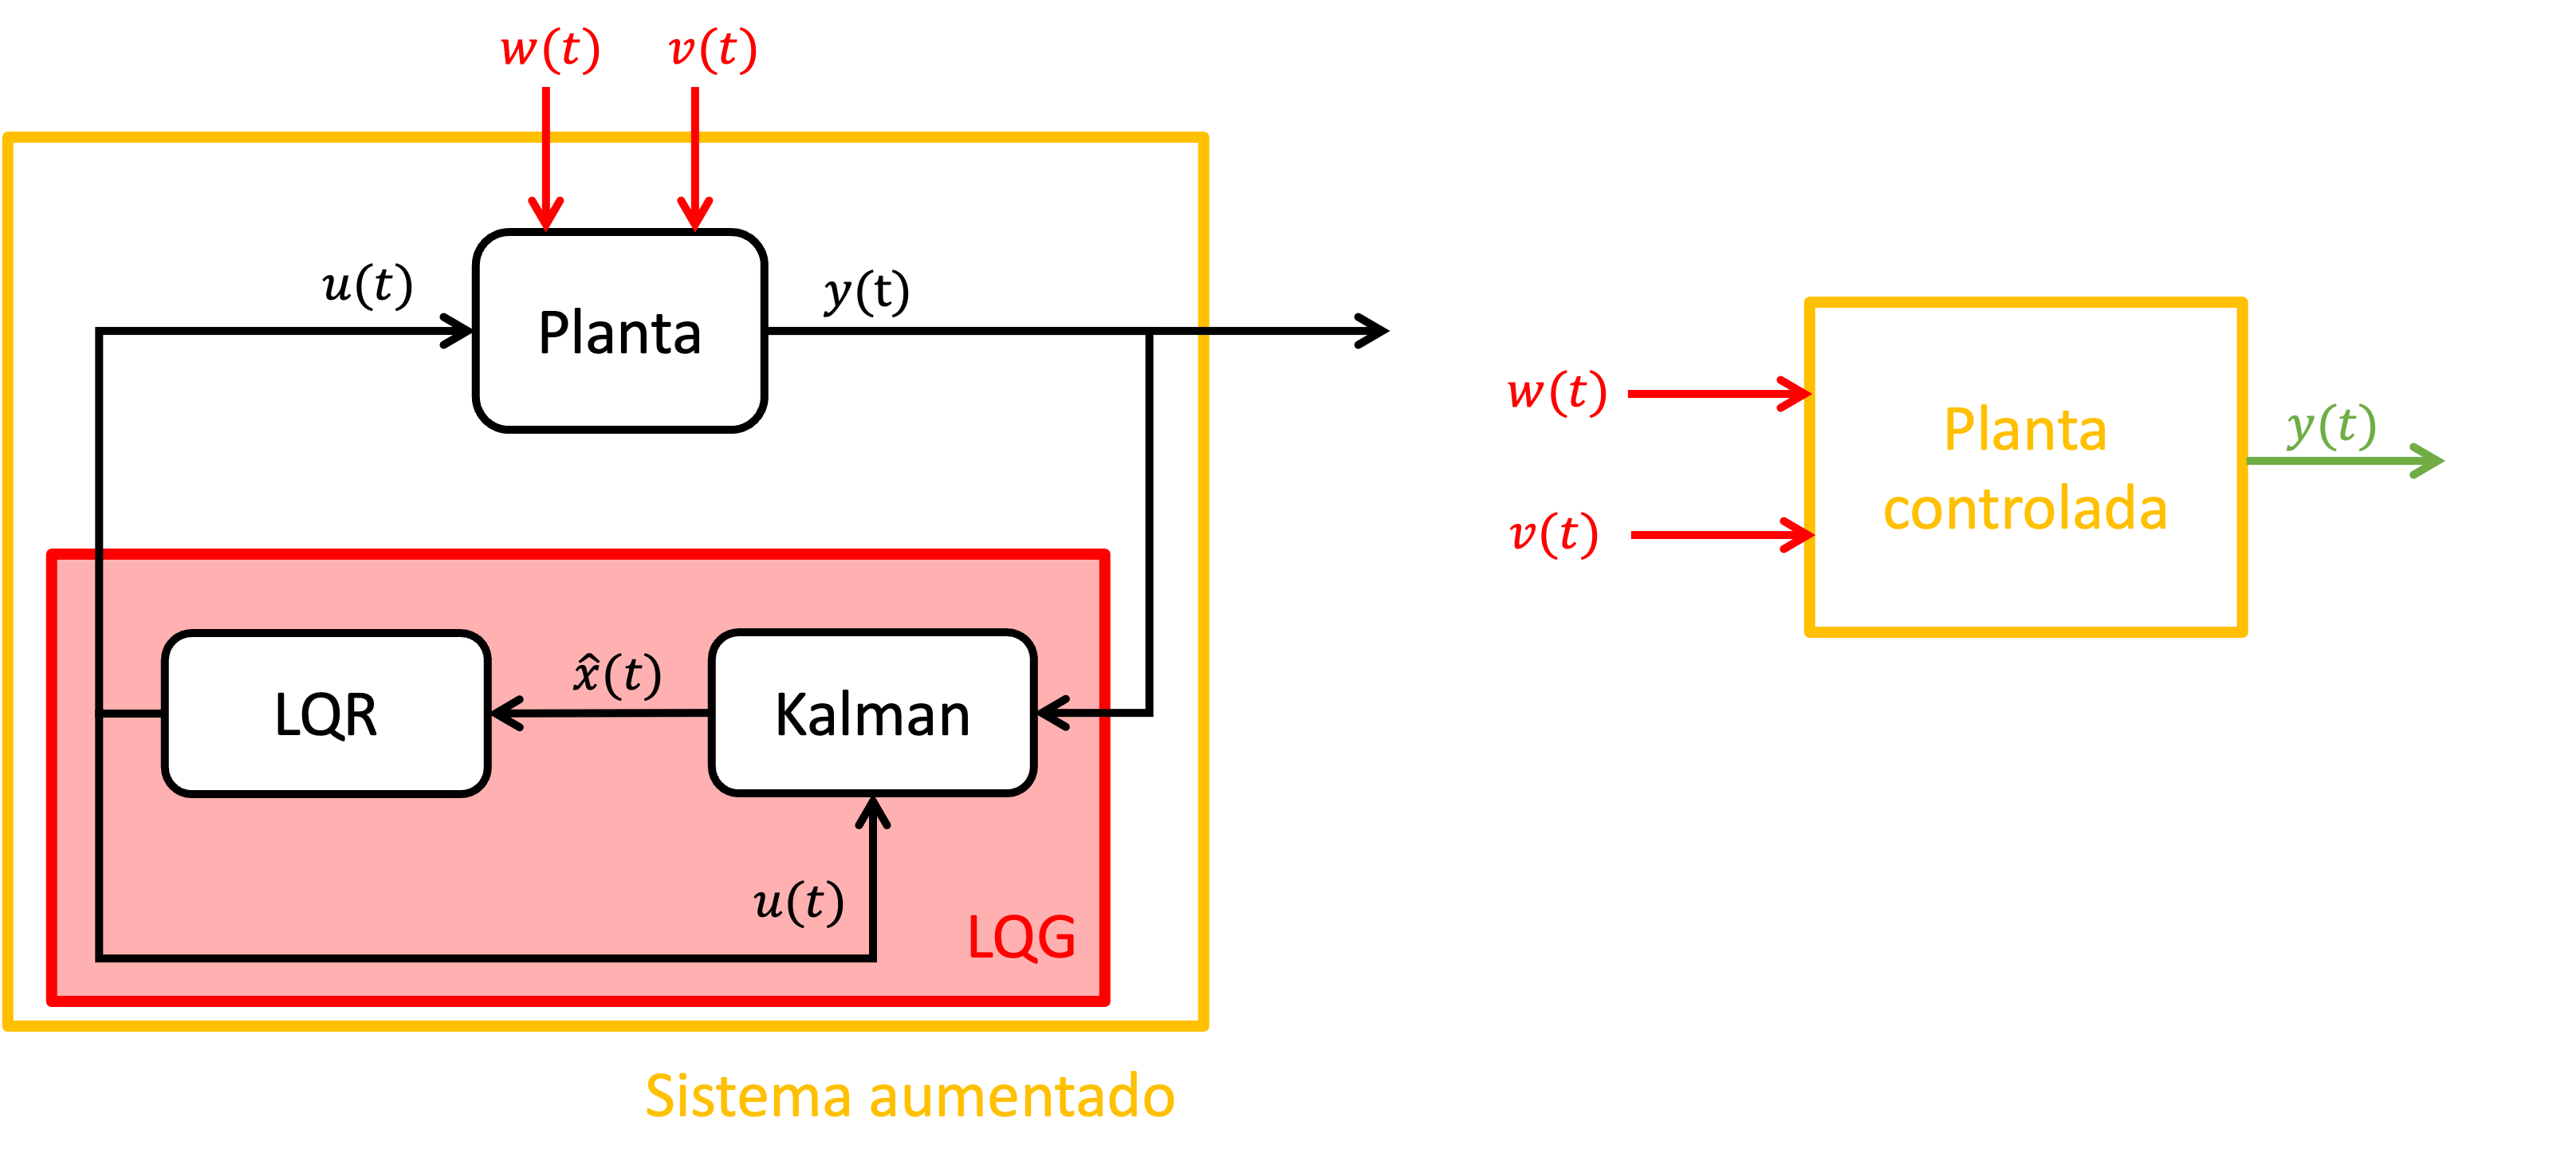
\includegraphics[scale=0.7]{Figuras/LQG.png}
\end{figure}

\underline{Parámetros LQG}: $Q$, $R$, $Q_w$, $R_v$.\\

